\section{Domain Specific Exceptions}\label{sec:DomainSpecificExceptions}
\bdq{Domain} means here a logical area of your product. You can translate it to \bsq{subsystem}, \bsq{component} or \bsq{module}, but of course also to \bsq{package}, \bsq{library} or even to \bsq{application} – whatever fits best for your purpose.

Each domain should have its \bdq{Domain specific Exception} – or, more precisely, its own, specific hierarchy of unchecked\index{exception!unchecked exception} or checked\index{exception!checked exception} (or both) exceptions, and for a complex product that may have more than one \bsq{domain}, you may end up with more than one hierarchy of \bdq{Domain Specific Exceptions}.

Internally, a domain could have also another hierarchy of (in this case checked) exceptions\index{exception!checked exception}, but these should not get visible outside that domain.

The biggest advantage of defining a hierarchy of domain specific exceptions is that it simplifies the public API of the domain it belongs to. An example for that would be the JDBC\index{JDBC} subsystem \autocite{ORACLE_DOC_SQL_PACKAGE,WIKIPEDIA:JDBC,DEV_TO:JDBC} whose methods are throwing only \lstinline|java.sql.SQLException|\index{java.sql!SQLException} \autocite{ORACLE_DOC_SQLEXCEPTION_CLASS} instances.

Except \lstinline|java.lang.IllegalArgumentException|\index{java.lang!IllegalArgumentException} and exceptions derived from that (\bdq{validation exceptions}, refer to chapter \tqref{sec:ValidationExceptions}, \hyperref[sec:ValidationExceptions]{above}), a domain may never emit an exception\index{exception} that is not defined by itself. All other exceptions (Exceptions, not Errors!) must be caught and handled or wrapped into an exception type specific to the current domain. The validation exceptions are thrown only by the methods that are part of the public API of the domain, as response of an invalid argument to that method. An \lstinline|IllegalArgumentException|\index{java.lang!IllegalArgumentException} that is thrown by another component used by this domain must be wrapped and delegated or handled internally.

To illustrate that, we assume that we defined the component \bdq{Print Support} in package \lstinline|com.jcc.printing| that should be responsible for the generation of documents for paper-like output and their distribution. It defines the exception class \lstinline|com.jcc.PrintingException| (or \lstinline|com.jcc.PrintingRuntimeException|, if you like that better), derived from \lstinline|java.lang.RuntimeException|\index{java.lang!RuntimeException}. It extends \lstinline|RuntimeException|\index{java.lang!RuntimeException} directly here, or if \bdq{Print Support} would be part of another domain (if it has a parent component), it will extend one of that component’s domain specific exceptions. Or there is an  \bdq{application exception} defined, so the domain specific exceptions will extend that.

To keep it simple, our \bdq{domain root exception} \lstinline|com.jcc.PrintingException| extends \lstinline|java.lang.RuntimeException|\index{java.lang!RuntimeException}; the full hierachy is shown in the class diagram on the next page\footnote{I have omitted the package names in the diagram to save space.}.
\clearpage

\begin{center}
% Generated by "dot -Tpng -y printingException.gv > printingException.png"
	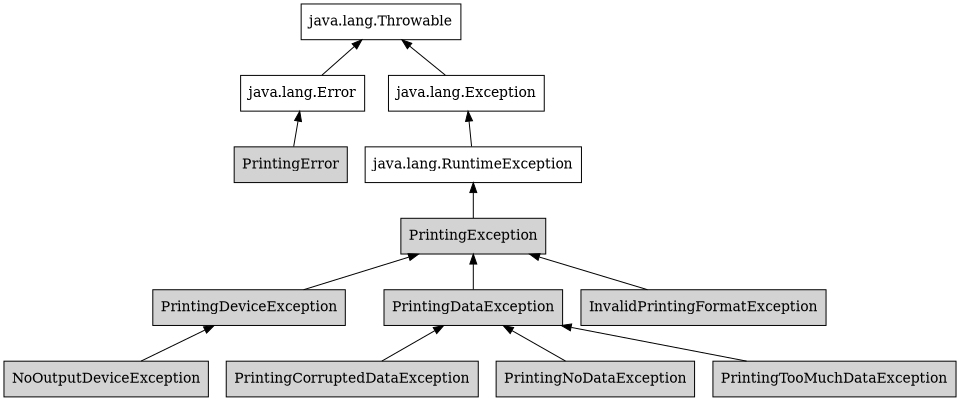
\includegraphics[scale=0.45]{coding/customExceptions/printingException}
\end{center}

The \bsq{domain root exception} \lstinline|PrintingException| allows all consumers of the \bdq{Print Support} component to catch all exceptions\index{exception} from that component with a single \lstinline|catch|\index{throw!catch} clause:
\begin{lstlisting}
try
{
    usePrinting( deviceId, … );
}
catch( final PrintingException e )
{
    final var message = """
````````printLetter(): Printing Operation failed!
````````Recipient Id: %s
````````Origin: %s
````````""".formatted( recipientID, dataSource );
    m_Loger.error( message, e );
    terminate();
}
\end{lstlisting}

\keeplisting{9}
Of course, instead of terminating (line~13, above) you can wrap message and exception into the appropriate domain specific exception of the consumer and throw that:
\begin{lstlisting}[firstnumber=4]
…
catch( final PrintingException e )
{
    final var message = """
````````Printing Operation failed!
````````Recipient Id: %s
````````Origin: %s
````````""".formatted( recipientID, dataSource );
    throw new <MyDomainSpecificException>( message, e );
}
\end{lstlisting}

In this sample, \bdq{\lstinline|recipientID|} and \bdq{\lstinline|dataSource|} enhance the information that is already provided with the \lstinline|PrintingException| object; probably the \bdq{Print Support} component was called with the data itself (not with the \bdq{\lstinline|dataSource|}), and the recipient is not part of the generated document.

The \bdq{Print Support} domain now defines problem specific exceptions derived from \lstinline|PrintingException|.

This allows the consumers of this component to respond to specific problems in an appropriate manner: if the \bdq{Print Support} component throws a \lstinline|PrintingDeviceException|, the consumer knows that there is a problem with the output device and can send an email to the support staff to inform them that the printer needs maintenance. A \lstinline|PrintingDataException| tells the consumer that the data they provided was faulty, and a \lstinline|PrintingTooMuchDataException| (derived from \lstinline|PrintingDataException|) signals that too much data was sent for printing. An \lstinline|InvalidPrintingFormatException| would indicate that the output description is not valid, and a \lstinline|NoOutputDeviceException| tells that there is no printer with the given name.

When the consumer wants to respond to all these exceptions differently\footnote{…~and they should do so! At least they should provide different data to the logging!}, the code snippet above needs to be changed to look like that below. Of course, we could always provide all information to the message when creating an instance of \lstinline|PrintingException| and leave it to the support engineer to identify what is relevant. But that would also mean that any kind of self-healing would get unnecessary complex.
\pslabel{listing:printingexceptions}
\begin{lstlisting}
try
{
    usePrinting( deviceId, … );
}
catch( final NoOutputDeviceException e ) // Self-Healing
{
    final var logMessage = """
````````printLetter(): Printing Operation failed because device does not exist
````````Attempting again with alternative device
````````Recipient Id: %s
````````Origin: %s
````````Missing Device: %s
````````Alternative Device: %s
````````""".formatted( recipientID, dataSource, missingDevice, getAlternativeDevice() );
    m_Logger.warn( logMessage, e );
    retryPrinting();
}(|\clearpage|)
catch( final InvalidPrintingFormatException e )
{
    final var exceptionMessage = """
````````Printing Operation failed due to an invalid format specification
````````Specification: %s
````````""".formatted( format );
    throw new IllegalArgumentException( exceptionMessage, e );
}
catch( final PrintingTooMuchDataException e )
{
    final var exceptionMessage = """
````````Printing Operation failed because a too large data set was sent for printing
````````Recipient Id: %s
````````Origin: %s
````````Data Size: %d records
````````""".formatted( recipientID, dataSource, dataSize );
    throw new <MyDomainSpecificException>( exceptionMessage, e );
}
catch( final PrintingDataException e )
{
    final var exceptionMessage = """
````````Printing Operation failed because the provided data set is invalid
````````Recipient Id: %s
````````Origin: %s
````````""".formatted( recipientID, dataSource );
    throw new <MyDomainSpecificOutputProblemException>( exceptionMessage, e );
}
catch( final PrintingException e )
{
    final var logMessage = """
````````printLetter(): Printing Operation failed with an unspecified error
````````Recipient Id: %s
````````Origin: %s
````````""".formatted( recipientID, dataSource );
    m_Logger.error( logMessage, e );
    abort();
}
\end{lstlisting}

The \bdq{Print Support} component signals that it cannot proceed by throwing a \lstinline|PrintingException| or one of the exceptions derived from it. What happens as response to that exception is on the consumer for that component: they could terminate the program, too, they could attempt to print again, they can choose an alternative mean to get the documents out, or they could even ignore the problem~… or they delegate the whole thing to its own consumers, by just wrapping the caught \lstinline|PrintingException| into its own domain specific exception – but this decision (\bdq{\textit{Either Log (and Terminate) or (Wrap and) Throw}}) must be made for each and every call.

Using an unchecked hierarchy\index{exception!unchecked exception} (the domain specific exceptions are extending \lstinline|java.lang.RuntimeException|\index{java.lang!RuntimeException}) means that the consumer can completely ignore the exception handling for the \lstinline|PrintingException|, leaving it to its own consumers.\footnote{It also means that the Java syntax does not require that the API methods for the \bdq{Print Support} component have a \lstinline|throws|\index{throw} clause, to declare the thrown exceptions – but this coding guideline demand that clause independent from the syntactical requirements.} The Bouncy Castle Crypto libraries\index{Bouncy Castle} \autocite{BouncyCastle,BouncyCastle:RuntimeCryptoException_CLASS} are an example for this approach\footnote{In fact, the Bouncy Castle libraries use both, unchecked and checked hierarchies.}.

The other approach, to use checked exceptions\index{exception!checked exception} (the domain exceptions extend \lstinline|java.lang.Exception|\index{java.lang!Exception}), can be found in the \lstinline|java.io|\index{java.io} \autocite{ORACLE_DOC_IO_PACKAGE} and \lstinline|java.nio|\index{java.nio} \autocite{ORACLE_DOC_NIO_PACKAGE} packages that define \lstinline|java.io.IOException|\index{java.io!IOException} \autocite{ORACLE_DOC_IOEXCEPTION_CLASS} as the \bdq{domain specific root exception} and derives exceptions like \lstinline|java.io.FileNotFoundException|\index{java.io!FileNotFoundException} \autocite{ORACLE_DOC_FILENOTFOUNDEXCEPTION_CLASS} from that.

Checked exceptions\index{exception!checked exception} enforce that each call to one of the component's method is somehow wrapped in a \texttt{try-catch}\index{try-catch-finally} block, otherwise the code does not compile. This forces attention for the error handling on each caller but it can also bloat the code. One can say, bloated code is much better than code without proper error handling, but when the code is too bloated with error handling stuff, it is difficult to read, and also prone to get broken when amended.

The parameter lists of the constructors\index{constructor} for the domain specific exceptions are not limited to the regular \lstinline|Throwable|\index{java.lang!Throwable} parameter for the \texttt{cause} and the \lstinline|String| parameter for the \texttt{message}. If there is a parameter that is required by each API method of the domain, this could be also a mandatory parameter for the domain specific Exception. For the \bdq{Print Support} component this could be the \texttt{id} for the output device. In that case, that \texttt{id} is no longer required to be part of the exception message argument for the constructor\index{constructor}.

If you add additional attributes to the domain specific exceptions, you should consider to add also getters\index{method!getter method} for these attributes, and you should override the method \lstinline|Throwable::getMessage|\index{java.lang!Throwable!getMessage()} \autocite{ORACLE_DOC_THROWABLE:getMessage} so that the additional attributes are part of the output when the exception object is printed somehow. Do not override the \lstinline|toString()|\index{java.lang!Object!toString()}\index{java.lang!Throwable!toString()} method in your new exception! When you have to do it (you must have very good reasons to do so!), make sure that the output format for the exception remains generally intact.

An example implementation of \lstinline|PrintingException| is shown on the following pages.
\clearpage
\begin{lstlisting}
package jcc.printing.exception;

import java.io.Serial;

import jcc.printing.DeviceId;
import jcc.printing.ErrorCode;

/**
 *  <p>{@summary The domain specific root exception for the Print Support
 *  component.}</p>
 */
public sealed class PrintingException extends RuntimeException
    permits InvalidPrintingFormatException, PrintingDataException, PrintingDeviceException
{
        /*------------*\
    ====** Attributes **==================================================
        \*------------*/
    /**
     *  <p>{@summary The id of the printing device that caused this
     *  exception.}</p>
     */
    private final DeviceId m_DeviceId;

    /**
     *  <p>{@summary The internal error code.}</p>
     */
    private final ErrorCode m_ErrorCode;

        /*------------------------*\
    ====** Static Initialisations **======================================
        \*------------------------*/
    /**
     *  The serial version UID for objects of this class: {@value}.
     *
     *  @hidden
     */
    @Serial
    private static final long serialVersionUID = 1174360235354917591L;

        /*--------------*\
    ====** Constructors **================================================
        \*--------------*/
    /**
     *  <p>{@summary Constructs a new {@code PrintingException} with 
     *  {@code null} as its detail message.} The 
     *  {@linkplain #getCause() cause} 
     *  is not initialised, and may subsequently be initialised by a call
     *  to 
     *  {@link #initCause}.</p>
     *  
     *  @param  errorCode   The internal error code.
     *  @param  deviceId    The printing device that caused this exception.
     */
    public PrintingException( final ErrorCode errorCode, final DeviceId deviceId )
    {
        super();
        m_DeviceId = requireNonNullArgument( deviceId, "deviceId" );
        m_ErrorCode = requireNonNullArgument( errorCode, "errorCode" );
    }   //  PrintingException()

    /**
     *  <p>{@summary Constructs a new {@code PrintingException} with the 
     *  specified detail message.} The 
     *  {@linkplain #getCause() cause} 
     *  is not initialised, and may subsequently be initialised by a call
     *  to 
     *  {@link #initCause}.</p>
     *
     *  @param  errorCode   The internal error code.
     *  @param  deviceId    The printing device that caused this exception.
     *  @param  message     The detail message. It is saved for later
     *      retrieval by the 
     *      {@link #getMessage()} 
     *      method.
     */
    public PrintingException( final ErrorCode errorCode, final DeviceId deviceId, final String message )
    {
        super( message );
        m_DeviceId = requireNonNullArgument( deviceId, "deviceId" );
        m_ErrorCode = requireNonNullArgument( errorCode, "errorCode" );
    }   //  PrintingException()

    /**
     *  <p>{@summary Constructs a new runtime exception with the specified 
     *  detail message and 
     *  {@linkplain #getCause() cause}.}</p>  
     *  <p>Note that the detail message associated with {@code cause} is 
     *  <i>not</i> automatically incorporated in this exception's detail 
     *  message.</p>
     *
     *  @param  errorCode   The internal error code.
     *  @param  deviceId    The printing device that caused this exception.
     *  @param message  The detail message (which is saved for later
     *      retrieval by the 
     *      {@link #getMessage()} 
     *      method).
     *  @param  cause   The cause (which is saved for later retrieval by
     *      the 
     *      {@link #getCause()}
     *      method). A {@code null} value is permitted,  and indicates
     *      that the cause is nonexistent or unknown.
     */
    public PrintingException( final ErrorCode errorCode, final DeviceId deviceId, final String message, final Throwable cause )
    {
        super( message, cause );
        m_DeviceId = requireNonNullArgument( deviceId, "deviceId" );
        m_ErrorCode = requireNonNullArgument( errorCode, "errorCode" );
    }   //  PrintingException()

        /*---------*\
    ====** Methods **=====================================================
        \*---------*/
    /**
     *  <p>{@summary Returns the id of the printing device that caused this
     *  exception.}</p>
     *
     *  @return The device id.
     */
    public final DeviceId getDeviceId() { return m_DeviceId; }

    /**
     *  <p>{@summary Returns the internal error code.}</p>
     *
     *  @return The error code.
     */
    public final ErrorCode getErrorCode() {return m_ErrorCode;}

    /**
     *  {@inheritDoc}
     */
    @Override
    public final String getMessage()
    {
        final var retValue = "%1$s - Error %2$s: %3$s".formatted( getDeviceId().getName(), getErrorCode().name(), mapFromNull( super.getMessage(), "<No Message>" ) );

        //---* Done *-----------------------------------------------------
        return retValue;
    }   //  getMessage()
}
//  class PrintingException
\end{lstlisting}

\bigskip

Some words regarding the calls to \lstinline|terminate()| vs. \lstinline|abort()| in the sample code on page \pageref{listing:printingexceptions}, \hyperref[listing:printingexceptions]{above}: assume we use the code snippet in a loop, where each cycle uses a different data set to be printed. A \lstinline|PrintingDataException| means that the current data set is somehow corrupted, but we can proceed with the loop (\textit{terminate} the current process and load the next data set), but an \lstinline|InvalidPrintingFormatException| or a \lstinline|PrintingDeviceException| means that no printing is possible at all and we \textit{abort} the loop by throwing the wrapper exception, and for the unspecific \lstinline|PrintingException|, even the consumer \textit{aborts}.

There are libraries that use \bdq{\lstinline|Error|} (domain specific implementations of \lstinline|java.lang.Error|\index{java.lang!Error}) to signal the abort condition, while \bdq{\lstinline|Exception|} means, \bdq{\textit{you can try again with different (valid) input data}}. It is a widely accepted best practice not to catch \lstinline|java.lang.Error|\index{java.lang!Error}, so we should not adopt this approach.

Nevertheless, you can of course define your \bdq{domain specific errors} and use them to signal really desastrous conditions that require to abort the program.

\bigskip

As already mentioned in chapter \tqfullref{sec:ValidationExceptions}, it is also possible to define specific validation exceptions\index{validation exception} for a domain, in addition to a hierarchy of regular exceptions.

The package \lstinline|java.util.regex|\index{java.util.regex} \autocite{ORACLE_DOC_REGEX_PACKAGE} (the regular expression handling in Java) is a sample for a domain that that manages with nothing but a domain-specific validation exception.

\bigskip

In large applications, either standalone\index{product type!standalone application} or server-based\index{product type!server-based application}, it is often observed that exceptions need to be caught on each level of the call chain, then wrapped into another exception, together with additional information. This could even mean that an exception is wrapped to another instance of the same class, just to add additional information.
\keeplisting{7}
\begin{lstlisting}
try
{
    …
}
catch( final PrintingException e )
{
    final var exceptionMessage = """
````````DataProcessor = %s\
````````""".formatted( dataProcessor.getName() );
    throw new PrintingException( e.getDeviceId(), e,getErrorCode(), exceptionMessage, e );
}
\end{lstlisting}

As we have seen in chapter \tqvref{sec:ExceptionCosts}, the creating of a new exception\index{exception} is not cheap. If it would be possible to add some information to the caught exception before it is re-thrown, these creation costs could be spared:
\keeplisting{4}
\begin{lstlisting}[firstnumber=5]
catch( final PrintingException e )
{
    e.addInfo( "DataProcessor", dataProcessor.getName() );
    throw e;
}
\end{lstlisting}

The source code for a wrapper exception as base class for domain specific exceptions is given in chapter \tqfullvref{code:WrapperException}.

%==============================================================================
% End of file!!
%==============================================================================
